\documentclass{beamer}
\usepackage{amsmath}
\usepackage{xcolor}
\usepackage{graphicx}
\usepackage{listings}
\usepackage{tikz}

\usetheme{default}
\usecolortheme{beaver}
\usefonttheme[onlymath]{serif}

\tikzstyle{startstop} = [rectangle, rounded corners, minimum width=3cm, minimum height=1cm,text centered, draw=black, fill=red!30]
\tikzstyle{arrow} = [thick,->,>=stealth]

\title{Utilizing reinforcement learning techniques to play Atari's Breakout}
\author{Andrew~Messing \and Ben~Brock \and Cory~Walker}
\date{November 24, 2015}
\subject{Computer Science}

\AtBeginSection[]
{
  \begin{frame}<beamer>{Outline}
    \tableofcontents[currentsection,currentsubsection]
  \end{frame}
}

\DeclareMathOperator*{\argmin}{arg\,min}
\DeclareMathOperator*{\argmax}{arg\,max}

\begin{document}

\begin{frame}
  \titlepage
\end{frame}

\begin{frame}{Outline}
  \tableofcontents
\end{frame}

% Section and subsections will appear in the presentation overview
% and table of contents.

\section{Breakout and Feature Extraction}
\begin{frame}{Breakout}
  \begin{itemize}
    \item Classic video game.  Developed by Atari.
  \end{itemize}
  \begin{center}
  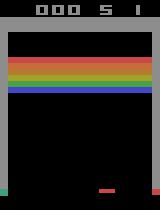
\includegraphics[width=50mm]{tmp.jpg}
  \end{center}
\end{frame}

\begin{frame}{Arcade Learning Environment}
  \begin{itemize}
    \item Simple object-oriented framework that allows researchers and hobbyists to develop AI agents for Atari 2600 games
    \item Allows access to each frame of the game and the ability to respond with an action
    \item Also allows access to number of lives remaining, score of the game, if gameover, etc
  \end{itemize}
\end{frame}

\begin{frame}{Actions}
  \begin{itemize}
  \item{Atari control is a joystick with a button on top and few menu buttons on the side}
  \item{20 possible actions including the buttons being pressed and the joystick being moved in 8 directions}
  \item{For breakout specifically we have 3 actions:}
    \begin{itemize}
      \item{Do nothing}
      \item{Move left}
      \item{Move right}
    \end{itemize}
  \end{itemize}
\end{frame}

\begin{frame}{Feature Extraction}
  \begin{itemize}
    \item{Image Processing to extract:}
    \begin{itemize}
      \item{Paddle's X position}
      \item{Ball's X position}
      \item{Ball's Y position}
    \end{itemize}
  \end{itemize}
  \begin{center}
  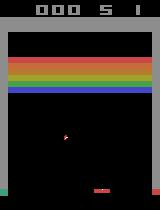
\includegraphics[scale=.75]{tmp2.jpg}
  \end{center}
\end{frame}

\section{Reinforcement learning}

\begin{frame}{Environment}
  \begin{itemize}
    \item Image processing module accepts a pixel representation of a Breakout session as input
    \item It outputs the coordinates of the paddle and ball
  \end{itemize}
  \vspace{2em}
  \begin{itemize}
    \item We choose $s = \text{ball}_{x} - \text{paddle}_{x}$ to determine the state
    \item $s > 0 \implies \text{the ball is to the right}$
    \item $s < 0 \implies \text{the ball is to the left}$
  \end{itemize}
  \vspace{2em}
  \begin{itemize}
    \item $s$ is mapped into a tabular state vector
  \end{itemize}
\end{frame}

\begin{frame}{Actions}
  \begin{itemize}
    \item Move the paddle left
    \item Move the paddle right
    \item Hold the paddle still
  \end{itemize}
\end{frame}

\begin{frame}{Rewards}
  \begin{itemize}
    \item -10 reward for losing the ball
  \end{itemize}
  \vspace{2em}
  \begin{itemize}
    \item This doesn't include rewards for eliminating blocks
    \item Will simply focusing on hitting the ball be enough to play the game well? (Yes!)
  \end{itemize}
\end{frame}

\begin{frame}{Pipeline}
  \centering
  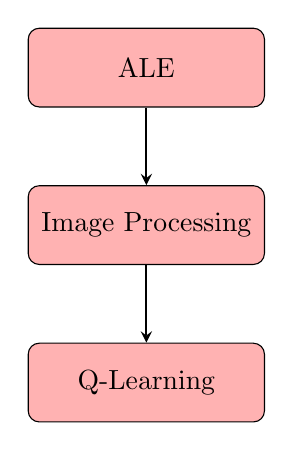
\begin{tikzpicture}[node distance=2cm]
    \node (ale) [startstop] {ALE};
    \node (start) [startstop, below of=ale] {Image Processing};
    \node (middle) [startstop, below of=start] {Q-Learning};
    \draw [arrow] (ale) -- (start);
    \draw [arrow] (start) -- (middle);
  \end{tikzpicture}
\end{frame}

\begin{frame}{Q-Learning}
  \begin{itemize}
    \item[] Initialize $Q(s, a)$ arbitrarily
    \item[] For each episode:
    \item[] \hspace{2em} $e(s, a) = 0$ for all $s, a$
    \item[] \hspace{2em} For each step:
    \item[] \hspace{4em} Discover current state $s$ with IP, choose action $a$
    \item[] \hspace{4em} Choose $a'$ for $s$ from $Q(s, a)$ ($\epsilon$-greedy)
    \item[] \hspace{4em} Take action $a'$, observe $r$ and $s'$
    \item[] \hspace{4em} $\delta = r + \gamma Q(s', a') - Q(s, a)$
    \item[] \hspace{4em} $e(s, a) = e(s, a) + 1$
    \item[] \hspace{4em} For all $s, a$:
    \item[] \hspace{6em} $Q(s, a) = Q(s, a) + \alpha \delta e(s, a)$
    \item[] \hspace{6em} $e(s) = \gamma \lambda e(s)$
    \item[] \hspace{4em} $s = s'$
  \end{itemize}
\end{frame}

\begin{frame}{Results}
  \begin{itemize}
    \item We don't have any yet!
    \item We will soon *fingers crossed*
    \item There will be cool graphs
  \end{itemize}
\end{frame}

\section{Deep reinforcement learning}

\begin{frame}{Problem definition}
  \begin{itemize}
  \item {
    Learn Atari games from raw pixels
  }
  \item {
    Google DeepMind
  }
  \item {
      Naive state space: $128^{210 \cdot 160} \approx 1.799\times 10^{70802}$
  }
  \item {
      Grayscale state space: $4^{210 \cdot 160} \approx 1.643\times 10^{20229}$
  }
  \item {
      Scaled grayscale state space: $4^{105 \cdot 80} \approx 2.013\times 10^{5057}$
  }
  \item {
    Still too huge
  }
  \item {
    And partially observable
  }
  \item {
    Generalization is essential
  }
  \end{itemize}
\end{frame}

\begin{frame}{Deep Q network}
  \begin{figure}[H]
    \centering
    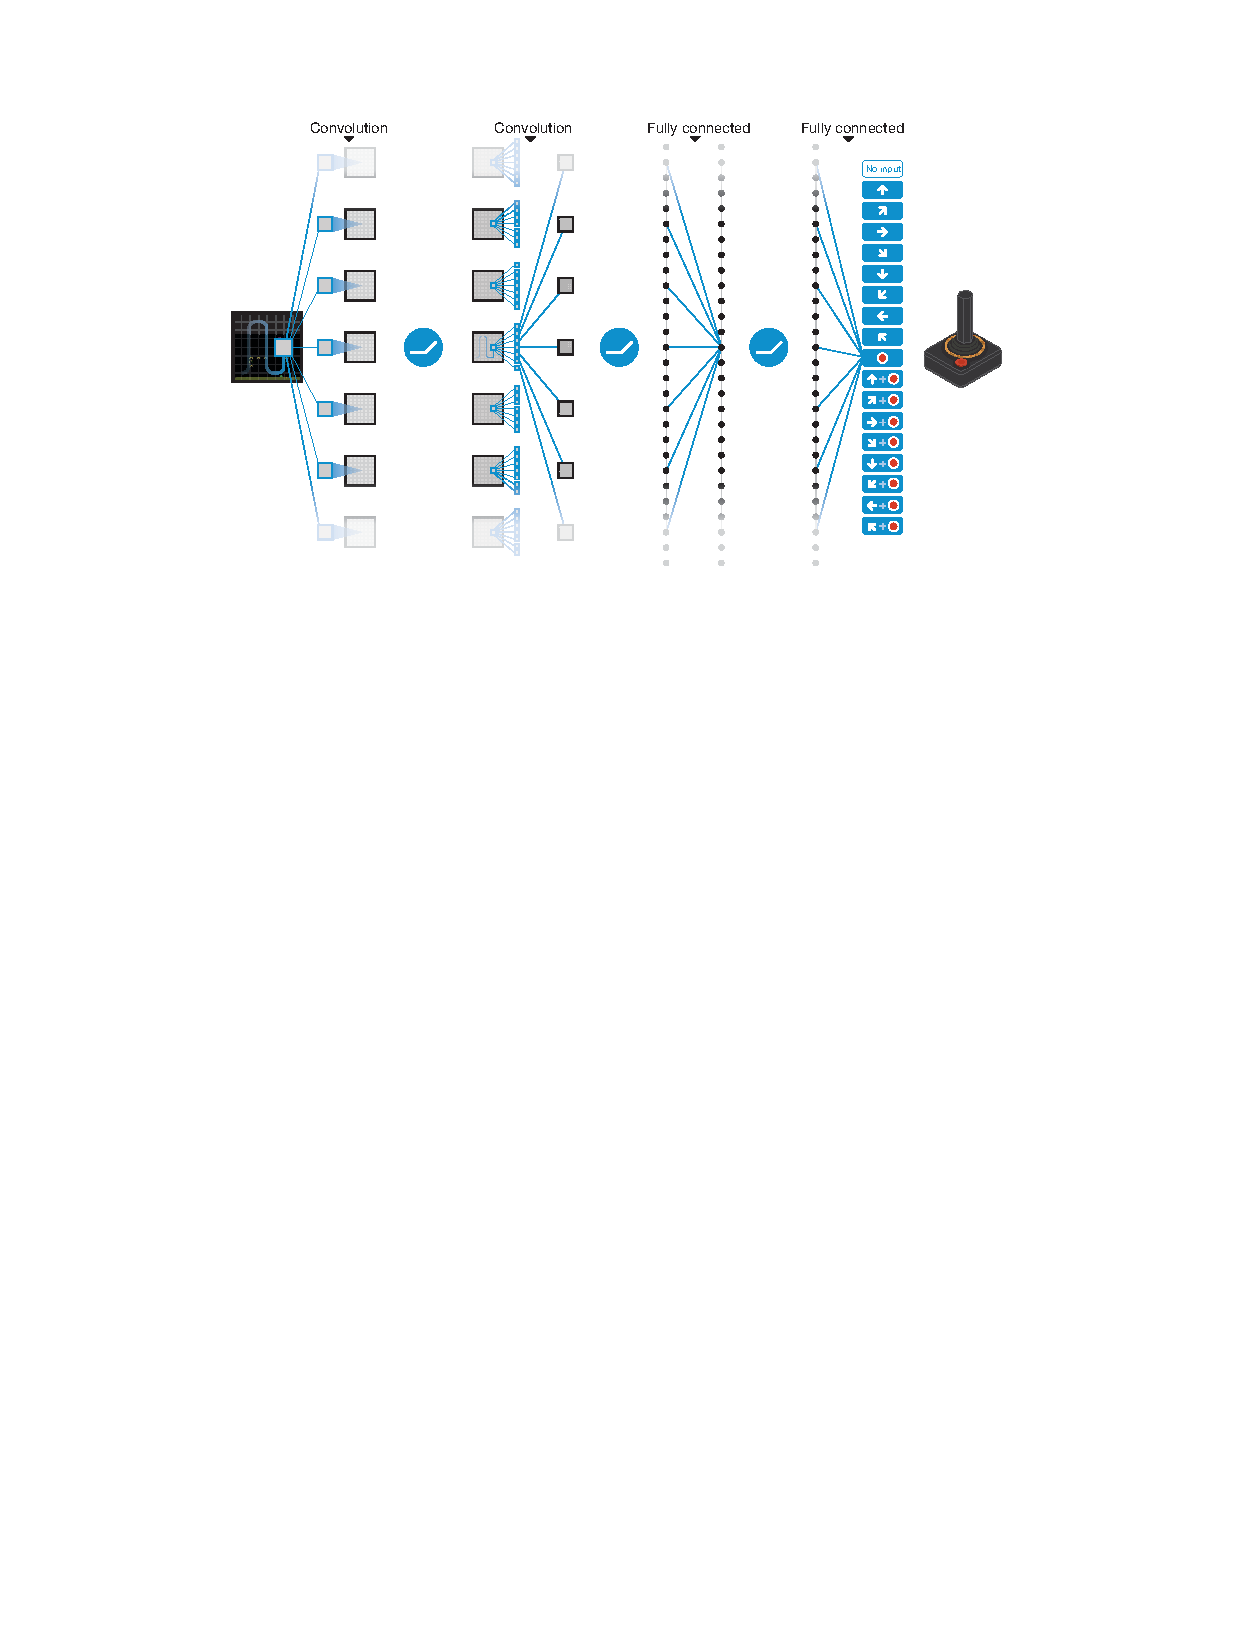
\includegraphics[width=105mm]{deep_q_network.pdf}
  \end{figure}
  \[ \boldsymbol{\theta}_{t+1} = \boldsymbol{\theta}_t+\alpha(Y_t^Q-Q(S_t,A_t;\boldsymbol{\theta}_t))\nabla_{\boldsymbol{\theta}_t}Q(S_t,A_t;\boldsymbol{\theta}_t) \]
\end{frame}

\begin{frame}{DQN variations}
  \begin{itemize}
  \item {
      NIPS (late 2013) - original paper from workshop, 24 hour training time
  }
  \item {
      Nature (early 2015) - similar to NIPS, more conservative hyperparameters (7 day training), model freezing
  }
  \item {
      Double DQN (September 2015) - branch from Nature model, attempts to address value overestimates
  }
  \end{itemize}
\end{frame}

\begin{frame}{Double DQN formulation}
  \begin{itemize}
    \item max operator means we use same values for action selection and evaluation, want to decouple.
    \item Action-value function has weights $\boldsymbol{\theta}_t$
    \item Target action-value function has weights $\boldsymbol{\theta}_t^-$
    \item After every 10,000 training updates, $\boldsymbol{\theta}_t^- \leftarrow \boldsymbol{\theta}_t$
  \end{itemize}

  \[Y_t^{\textrm{DQN}} \equiv R_{t+1} + \gamma \textcolor{red}{\max_{a} Q(S_{t+1},a;\boldsymbol{\theta}_t^-)} \]
  \[ \Downarrow \]
  \[\boxed{Y_t^{\textrm{DoubleDQN}} \equiv R_{t+1} + \gamma \textcolor{red}{Q(S_{t+1},\argmax_a Q(S_{t+1},a;\boldsymbol{\theta}_t),\boldsymbol{\theta}_t^-)}} \]
  \begin{itemize}
    \item If $\boldsymbol{\theta}_t^- = \boldsymbol{\theta}_t$ (NIPS model), no difference
  \end{itemize}
\end{frame}

\begin{frame}{Implementation}
  \begin{itemize}
    \item Nathan Sprague, \href{https://github.com/spragunr/deep_q_rl}{https://github.com/spragunr/deep\_q\_rl}
    \item Circular buffer for 1M replay frames, visualization code, model saving and loading
    \item Already supported NIPS and Nature algorithms.
    \item After some Theano debugging, my fork now supports Double DQN
    \item EC2 g2.2xlarge
    \item Single threaded, CPU bound, 30\% GPU utilization, 8GB replay buffer
  \end{itemize}
\end{frame}

\begin{frame}{Double DQN Results}
  \begin{figure}[H]
    \centering
    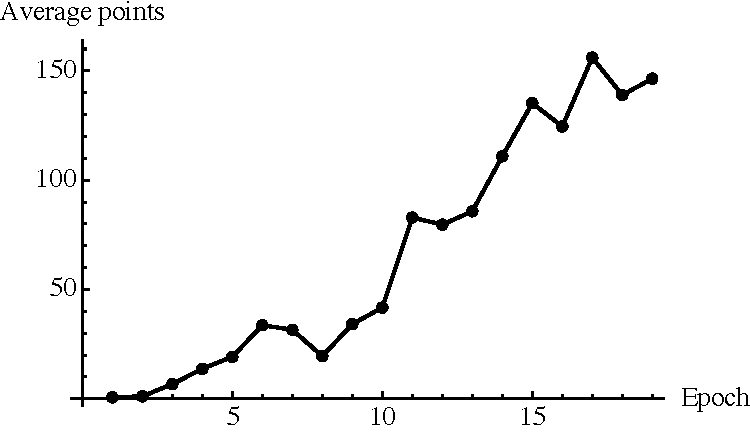
\includegraphics[width=90mm]{dqn_rewardper.pdf}
  \end{figure}
  Each epoch takes about an hour. Stopped after $\sim 20$ hours.\\
  \vspace{12pt}
  \url{https://youtu.be/UXurvvDY93o?t=5m21s}
\end{frame}

\begin{frame}{Double DQN Results}
  \begin{figure}[H]
    \centering
    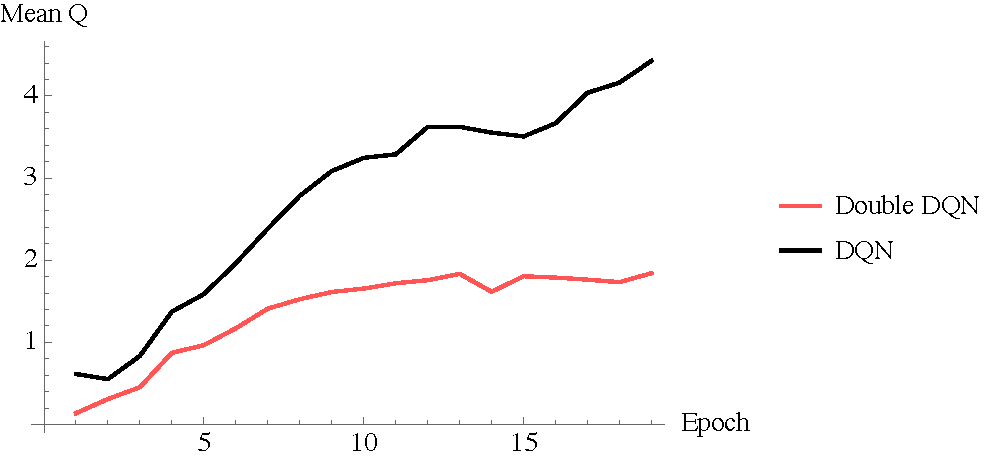
\includegraphics[width=90mm]{dqn_meanq.pdf}
  \end{figure}
\end{frame}


% Placing a * after \section means it will not show in the
% outline or table of contents.
\section*{Summary}

\begin{frame}{Summary}
  \begin{itemize}
  \item
    With the right kind of feature extraction, problem simplifies.
  \item
    A pixel-based learning algorithm is slow to train but generalizable.
  \item
    DQNs struggle with certian types of problems.
  \end{itemize}
  
\end{frame}


% All of the following is optional and typically not needed. 
\appendix
\section<presentation>*{\appendixname}
\subsection<presentation>*{For Further Reading}

\begin{frame}[allowframebreaks]
  \frametitle<presentation>{For Further Reading}

  \begin{thebibliography}{10}

  \beamertemplatebookbibitems

  \bibitem{suttonbarto}
    Sutton, R. S., \& Barto, A. G. (1998). \textit{Reinforcement learning: An introduction} (Vol. 1, No. 1). Cambridge: MIT press.

  \beamertemplatearticlebibitems

  \bibitem{dmnips}
    Mnih, V., Kavukcuoglu, K., Silver, D., Graves, A., Antonoglou, I., Wierstra, D., \& Riedmiller, M. (2013). Playing Atari with deep reinforcement learning. \textit{arXiv preprint arXiv:1312.5602}.

  \bibitem{dmdoubl}
    van Hasselt, H., Guez, A., \& Silver, D. (2015). Deep Reinforcement Learning with Double Q-learning. \textit{arXiv preprint arXiv:1509.06461}.
  \end{thebibliography}
\end{frame}

\end{document}
